This option allows users to determine the event at the base of the 
building by first performing an effective free-field  site response 
analysis of a soil column. In this panel the user specifies a ground 
motion at the bottom of the column. With the soil layers properly 
defined, the motion at the ground surface will be given at the end 
of the analysis and this is the motion that will be used in the 
simulation of the building response. 

\begin{figure}[!htbp]
  \centering {
    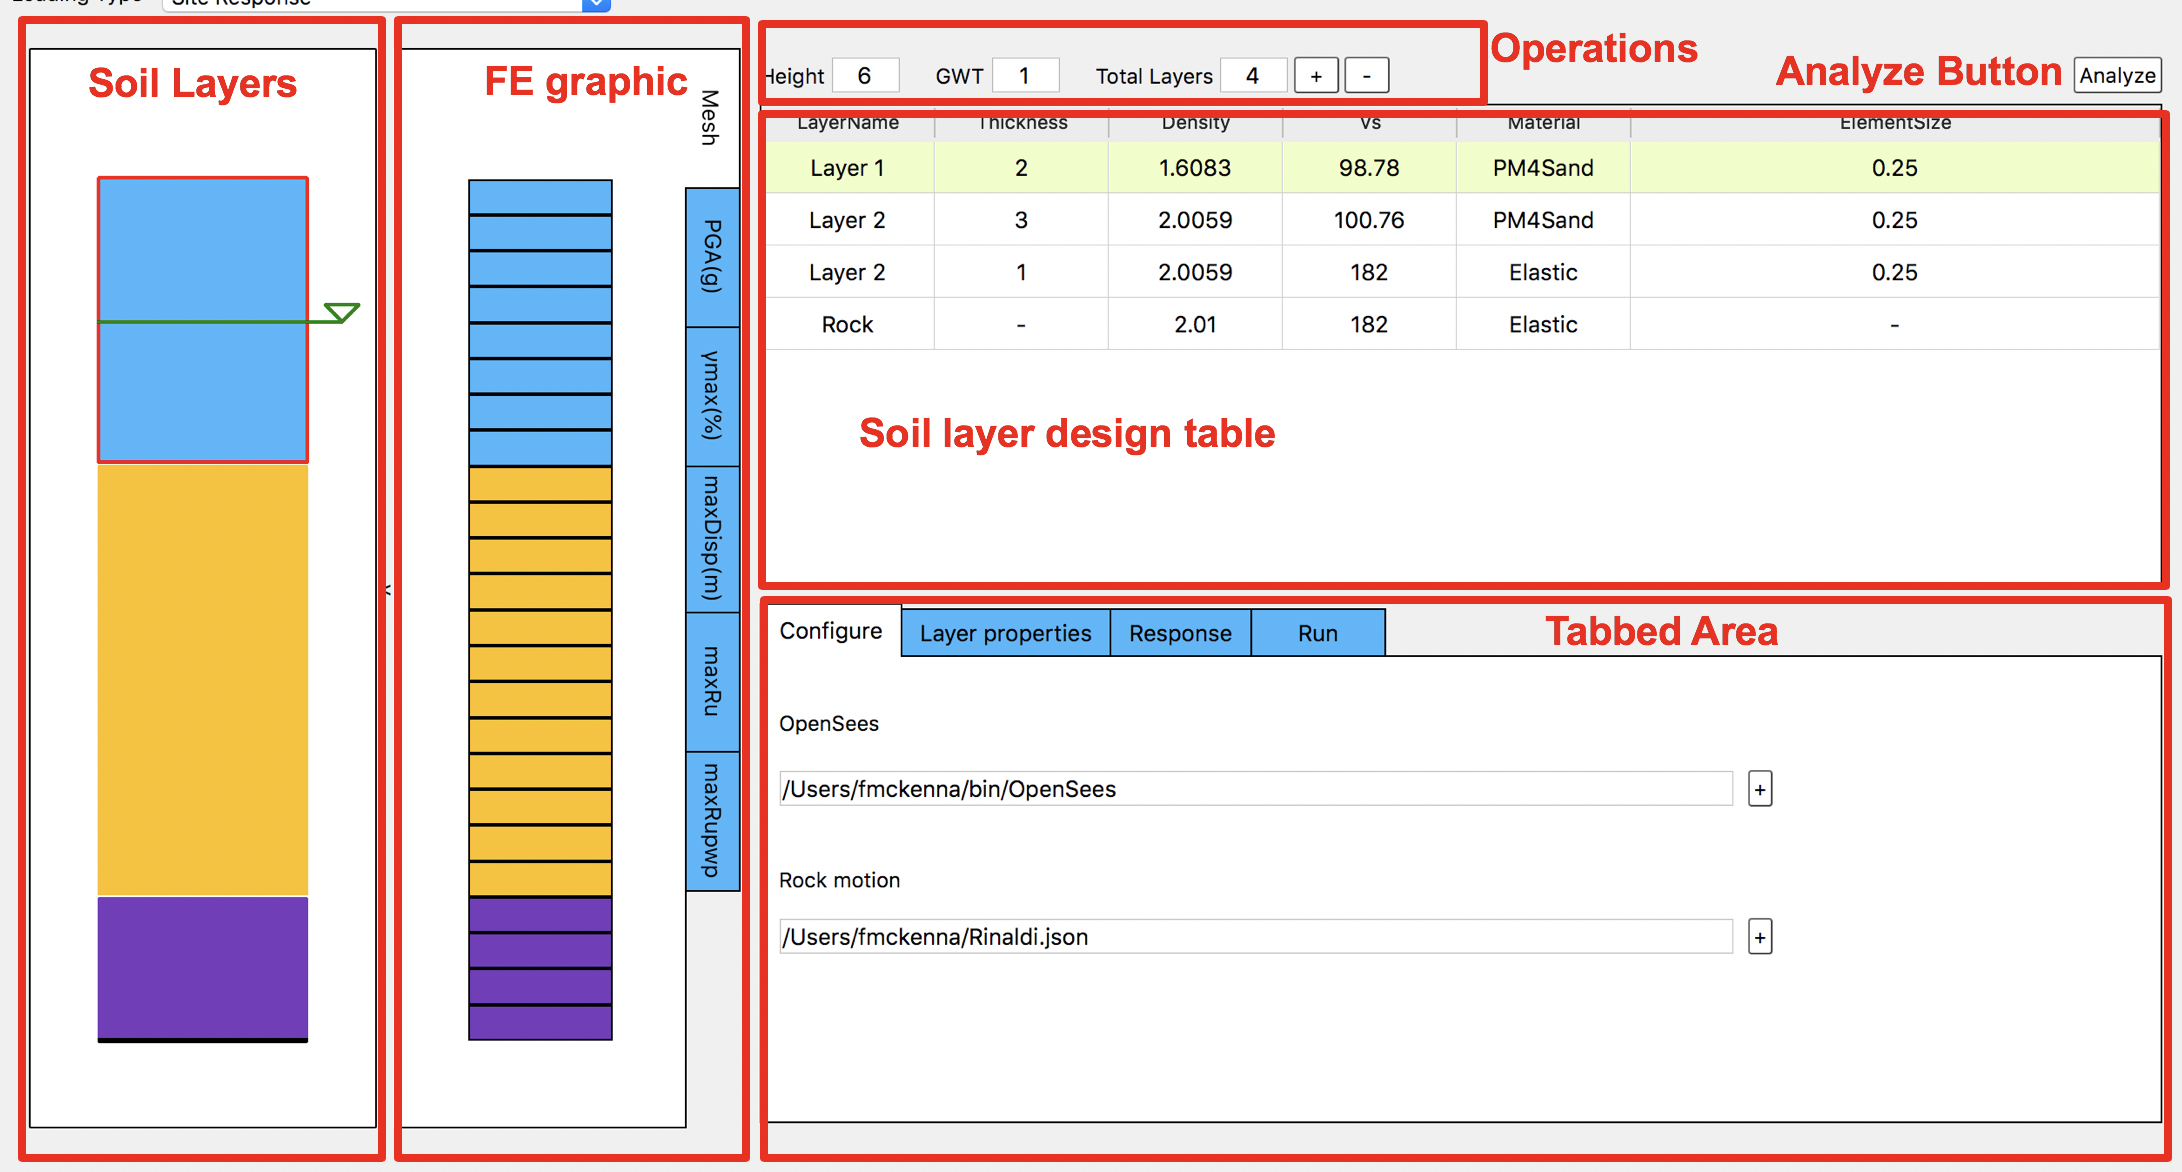
\includegraphics[width=0.8\textwidth]
    {usage/figures/s3hark1.png} }
  \caption{Site Response Analysis Event}
  \label{fig:s3hark1}
\end{figure}

The UI of the Site Response is shown in \Cref{fig:s3hark1}. It is split into a number of areas:
\begin{enumerate}
\item Soil Column Graphic: The first graphic on the left of the panel is 
the soil column graphic, which shows a visualization of the soil column.
\item FE Mesh Graphic: The second graphic is the mesh graphic, which shows 
the finite element mesh and profile plots. Selecting any of the tabs on the right inside this graphic (PGA, Vmax, maxDisp, maxRu, maxRuPWP) will show results
from the simulation at the mesh points for the different options.
\item Operations Area: The right side of this show some information, e.g. Height and number of soil layers, and includes plus and minus buttons. If the user presses the plus button, a layer will be added below the current selected layer. If the minus button is pressed the current selected layer will be removed.

Also in the operations layer is the Ground Water Table (GWT) line edit where the user edits the level of the ground water table and a button Analyze. The analyze button is performed to run the simulation locally so that the user can review the motion predicted at the surface.
\item Soil Layer Table: This table is where the user provides basic information on the soil layer, including layer thickness, density, vs30, material type, and element size in the finite element mesh.
\item Tabbed Area: This contains a number of tabbed widgets: \begin{enumerate}
\item Configure Tab: In the configure tab, both the path to the OpenSees executable and rock motion file are entered by the user. The rock motion file must currently be in SimCenter event format, a number of examples of which are available with the source code. \href{https://github.com/NHERI-SimCenter/EE-UQ/tree/master/example1/event}{(example source code)} 
\item Layer Properties Tab: For the selected layer, the user enters additional material properties as shown in \Cref{fig:s3hark3}.
\item Response Tab: Once the site response analysis has been performed, the user can enter this tab and review element and nodal time varying respone quantaties.
\item Run Tab: Opens up a window in which by using the up and down arrows on the keyboard the dino will jump up and down. Something to do if the site response analysis is taking too long, which it may if many layers of PM4sand is used.
\end{enumerate}
\item Analyze Button:
The user clicks the Analyze button to start the finite element analysis. Once clicked a progress bar will show the status. When done if the user selects the Response in the tabbed area they will be able to review the results.
\end{enumerate}

\begin{figure}[!htbp]
  \centering {
    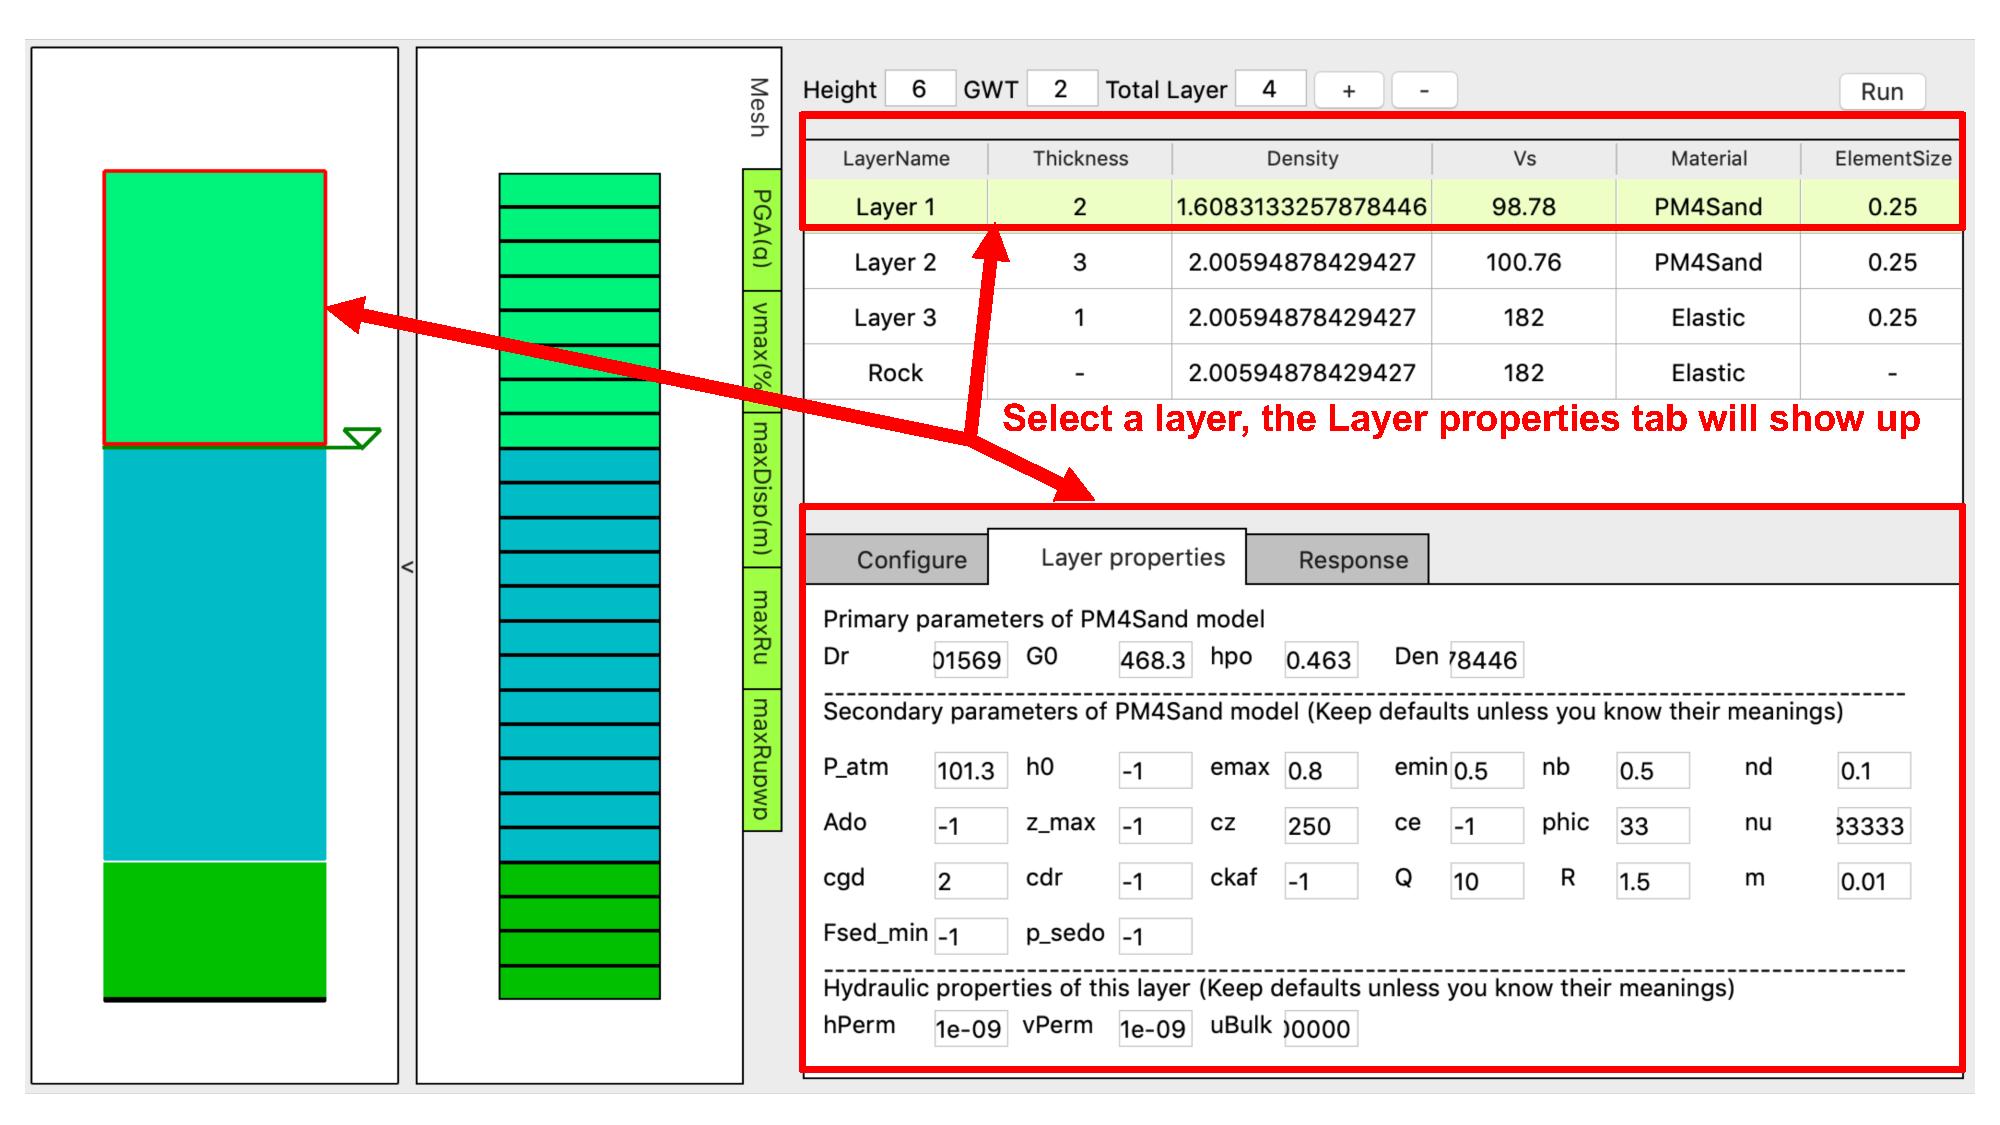
\includegraphics[width=0.8\textwidth]
    {usage/figures/s3hark3.pdf} }
  \caption{Soil Layer Modification in Site Response }
  \label{fig:s3hark3}
\end{figure}

Upon the finish of the finite element analysis, the ground motion at the soil surface (\Cref{fig:s3hark4}) will be stored in EE-UQ's input file.
This computed motion will be later applied to the bottom of the building.

Random Variables: In this version, no inputs may be selected as being random variables.\\

NOTES: 
\begin{enumerate}
\item All units are in m, kPa, and kN when entering inputs in the Site Response panel.
\item If the Analyze button is not pressed no simulation will be performed. If no simulation is performed there will be no ground motions provided to the building.
\end{enumerate}
